
According to IDC (www.idc.com) -- a global provider of market intelligence, advisory services, and events for the information technology, telecommunications and consumer technology markets -- the worldwide shipment of smart connected devices will surpass 2.5 billion units in 2017. The decreasing trends of cost, size, and power requirements of the various devices, were accompanied by an increase in embedded computing capabilities. In addition -- every device can be connected with other devices, each of which: (1) is capable of sensing/computing, communicating and actuating; (2) depends on values and state-descriptions of other devices, not necessarily within geo-spatial proximity nor with homogeneous physical characteristics, to steer the course of its own activities.  Such heterogeneous device range from computers, tablets and smartphones, through embedded systems in cars and traffic lights, precision agriculture sensors and actuators, to various home appliances, bodily sensors, etc.~\cite{Al-FuqahaGMAA15,AtzoriIM10,MelodiaPGA07,SalarianCN12}. According to recent a study by Goldman \& Sachs, over 12 billion devices are already connected to the Internet of Thing (IoT) and by 2020 that number should become 20 billion~\footnote{http://www.goldmansachs.com/our-thinking/pages/iot-meets-everything.html}.

%%People and data are already online. Soon, all sort of things with sensors, actuators and places will be also online. All sectors of activity will %%benefit from applications that leverage the interconnection of embedded systems with IT systems. Intelligent transport solutions can speed up %%traffic flows, reduce fuel consumption, and safe lives. Smart farming solutions will improve the production and delivery of safe and healthy food. %%Remote health monitoring will provide convenient access to healthcare, raises it quality, and save money. Utilities management, education, %%government services, retail sectors etc.… all will also benefit from such couplings and the things will leave across all different systems. %%\textbf{The next step is to interconnect these individual systems into a system of systems, and here we are confronted to such a scale and %%heterogeneity that we are reaching a limit in networking and software engineering}.\\

Recent works have already attempted to capitalize on the results from social networks research~\cite{AhmedEH15,Hai-Jew16,MorrisTP10,VenturiniJL15} -- namely~\cite{AtzoriCI14,IeraMA15} have specifically pointed how the experiences from social networks of users equipped with smart devices could be generalized to {\it social networks of devices} in the IoT realm. In a similar spirit, attempts have been made to demonstrate the benefits of {\it virtual objects} as a good abstraction for tackling IoT-related problems~\cite{NittiPCA16}. Studies regarding integration of heterogeneous devices in various contexts abound -- e.g., from smart homes in a manner that would balance the Quality of Experience (QoE) and Energy consumption~\cite{FlorisMPA15}; to better use of smart grid~\cite{LuoAM14} and enabling smart cities~\cite{ZanellaBCVZ14}.

One of the core motivations for the proposed project is based on the observation that current practices related to the design of IoT systems are still rather compartmentalized, and the dynamics-aware fusion of data collection, analytics processing and actuation across a variety of heterogeneous IoTs has limited support. As a simple example, consider a scenario where one has a (collection of) smart bed(s), such as, e.g., RestBed (https://www.restperformance.com/) with a surface equipped with multiple sensors to improve sleeping experience. A smart home may, in addition to a RestBed, also have smart refrigerators such as, e.g., Family Hub from Samsung (http://www.samsung.com/us/explore/family-hub-refrigerator/). While the QoE estimate can be obtained based on customers survey (or, even from bodily sensors), and it can even be balanced with the energy-efficiency (cf.~\cite{FlorisMPA15}) ``in-concert'' with such devices, there are some important functionalities that are lacking, and could yet significantly improve the overall experience and efficient use of the available devices/technology:

\begin{itemize}
\item The quality/satisfaction of sleeping is not correlated with the nutritional habits (i.e., the content of the food in the smart refrigerator and consumption patterns). This, in turn, prevents the respective manufacturers from improving their products/devices in a collaborative and context-aware manner.

\item There is no formal methodology of {\it where} the data assembling (as well as data aggregation and decision/recommendation as well as actuation) should take place. For instance, should all the nutrition-relevant data from an ensemble of smart refrigerators be sent at the local grocery store to optimize deliveries, or should it be aggregated at some geo-social level of hierarchy. Moreover, this raises the question of how the aspects of privacy and security should be handled.
\end{itemize}



%In this project, we aim to investigate issues related to the design and development of a secure physical and computational networked environment, %consisting of a large collection of connected smart objects (things). The proposed environment would allow interoperability and would also %facilitate efficient collection and processing of data from these {\it things} and development of analytics based on the collected data. Based on %these analytics, the {\it things} would be able to relate to each other to form dynamic networks (akin to social networks, in this case, of {\it %things}). These smart objects may come from diverse environments such as smart appliances at homes, smart mobile surveillance system such as fire %trucks and police cars, smart transportation entities (e.g., cabs or buses), etc.



%Nowadays, existing start of the art related to the design of IoT systems is highly compartmentalized, the data collection and analytics processing %across a variety of heterogeneous IoTs has limited support, and the interoperability of objects across domains has not been addressed at a level %that would provide the kinds of optimizations that this project aims to achieve. In this project, we introduce the concept of collaborative Social %Network of Things that would enable data and analytics sharing across objects that exhibit similar operating characteristics and/or have similar %profiles in terms of usage and user/manufacturer parameters. In addition, we propose to develop a hierarchical middleware implemented as fogs to allow interoperability with context-aware security properties associated with different nodes. These middleware fogs, mainly implemented in smart boxes/gateways within local networks, will manage the communication between the associated smart objects and the network in an optimized way that takes into account both the characteristics of the smart objects and the preferences of the users. The massive generated data by all these connected smart objects and stored in the system will enable the cognitive network, through deep learning algorithms, to raise dynamic procedures that will enable a multi-criteria optimizations of the  behavior  of these smart objects.\\

 Extending the above scenario, one may consider an evolution along spatio-temporal dimension. For instance, during a lunch-break, Jack decides to lower by 5F the set temperature of his home heating system – to activate when he is less than 1 mile from his home and in any case no later than 6PM. However, if the outside temperature drops below 55F, the home temperature must go up by 5 degrees. A colleague gives Jack a list of instructions corresponding to a new method for washing wool sweaters; he  sends the file directly to his home through the social network where a service will adapt the instructions to his washing machine’s particular technical features and his personal preferences (e.g., extra soft cloths). % Back at home, Jack launches “my angry day” profile through  smartphone, which automatically dims the light and has the Hi-Fi play his favorite relaxing music. Meanwhile,
  At home a tip from the network tells Jack to turn off all TVs to avoid getting further depressed. During the night the washing machine starts the cycle at the time the electric company informs it to be the most favorable.

%%\begin{wrapfigure}{R}{0.60\textwidth} \vspace{-3mm}
%%	\centerline{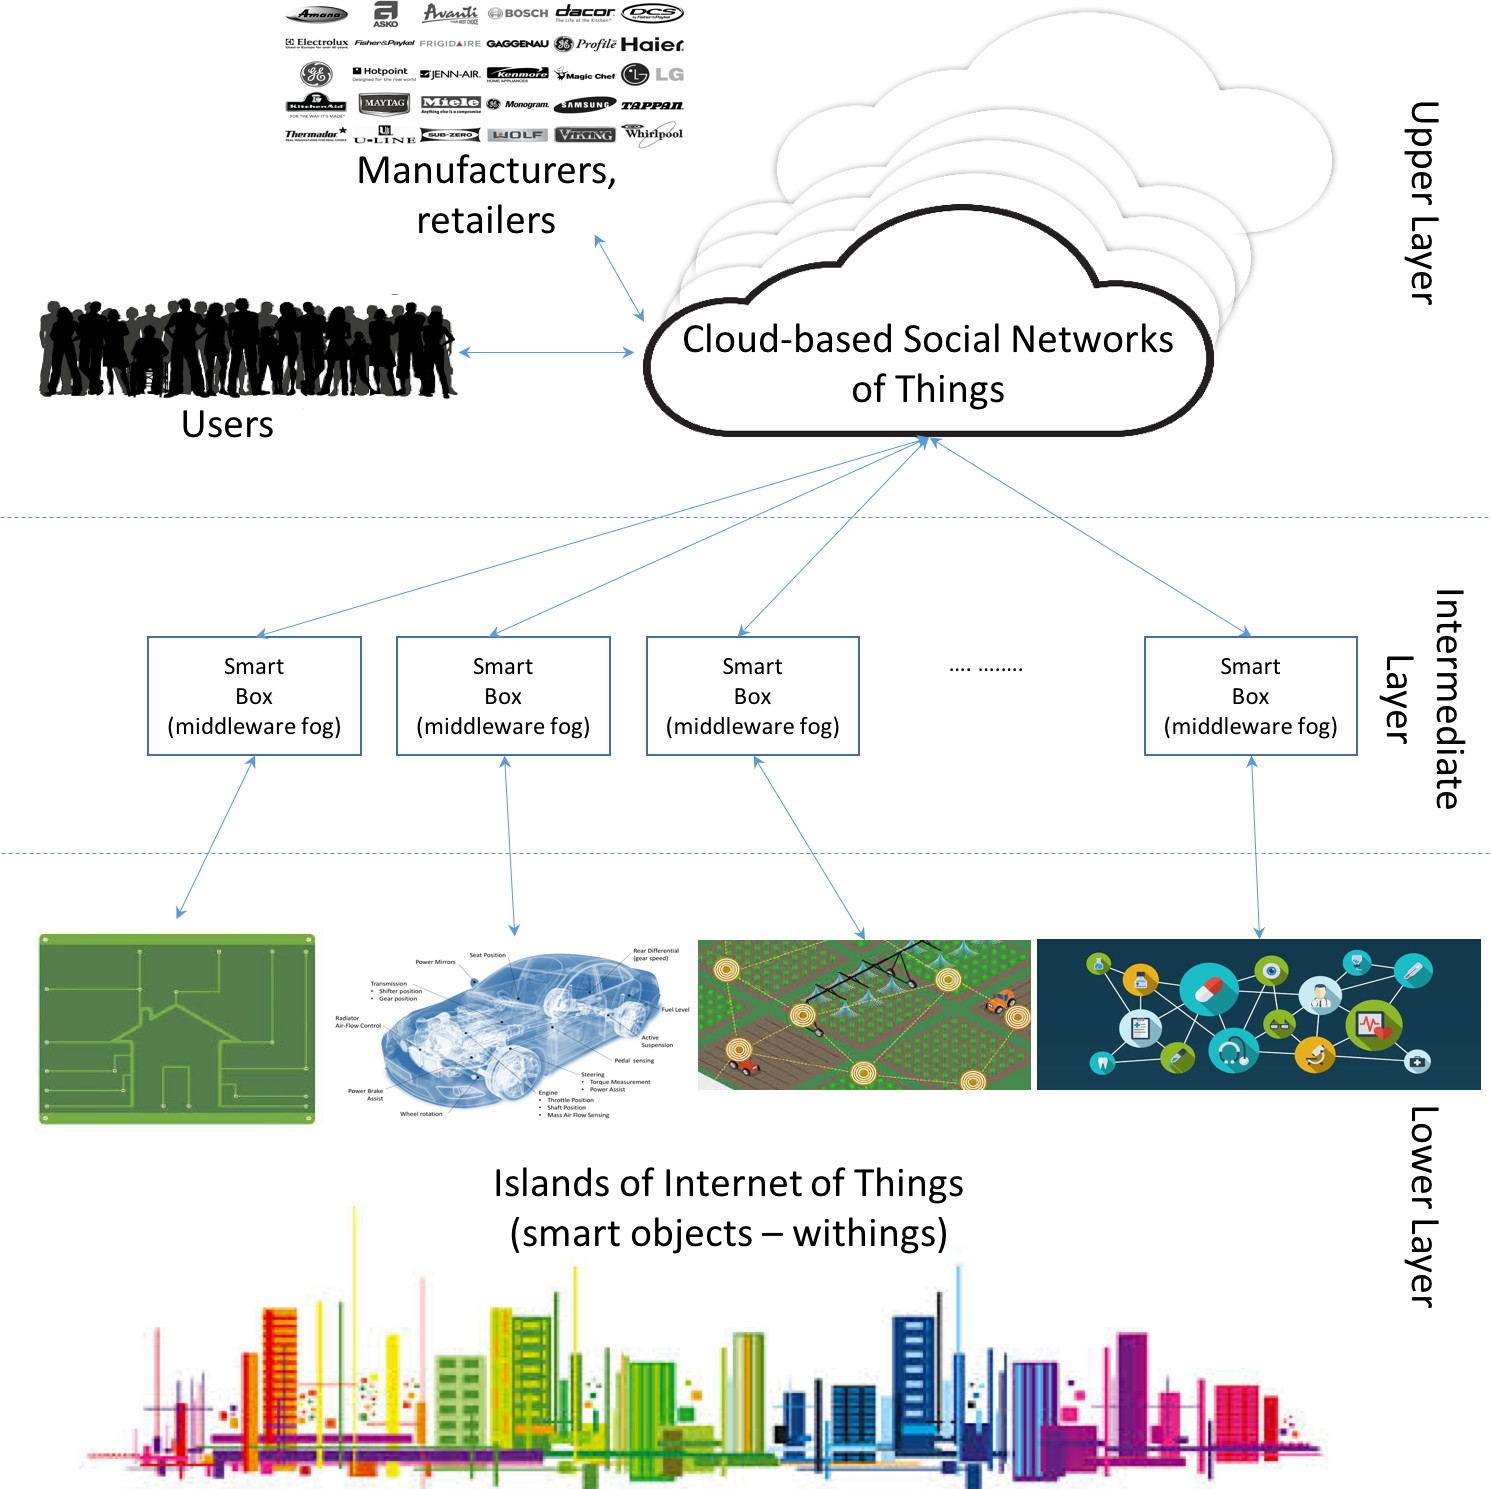
\includegraphics[width=0.60\textwidth]{./fig1.png}}
%%	\vspace{-3mm} \caption{\small Depiction of the proposed system}
%%	\label{fig1}
%%	\vspace{-3mm}
%%\end{wrapfigure}

The above describes a single user interacting seamlessly with multiple devices. We observe that one could attempt to generalize the existing approaches for Social Network of Things~\cite{IeraMA15,NittiPCA16} that can be generated/organized and dissolved on-the-fly, and enable scalability.
 %where different criteria can be used to orchestrate the behavior of (groups of) instances subject to multiple constraints; and certain security and privacy concerns are ensured.
However, even in the context of ``Jack'' scenario, there are certain aspects that span across heterogeneous domains/types and at different levels of certain (e.g., hierarchical) relationships. For instance, collaboratively regulating the temperature with other units in Jaack’s building has one kind of spatial, temporal, and devices extent, whereas collaboratively deciding about the cycle of the washing machine may go beyond the building -- i.e., optimizng grid-demand within a city-block.
%adjusting the Hi-Fi themes based on the fact that Jack decided to join his co-workers for a happy-hour; etc…

By establishing a dynamic instantiations of various components/devices comprising Internet of Things (IoT) structures, we aim to  provide an automatic resource optimization and other intelligence into these evolving collections of smart connected objects, going beyond the social networks of things. Rather than endowing them with autonomously cognitive chips, we aim to enable manufacturers, retailers and users/owners, to elaborate finely tuned dispatches to be distributed toward the smart objects through {\it middleware fogs} located various units (e.g., homes).
As part of the proposed research we plan to provide novel data analytics methodologies that will: (a) incorporate the fact that some users may not be cooperative in terms of suggested regime of use for certain devices/task; (b) provide a specific behavioral insights to be used by various manufacturers when planning the design of certain devices so that they can be better adapted to changing conditions of use.
 A high-level description of the architecture we target to develop for supporting such  scenarios is depicted in Figure~\ref{fig1}, providing methodologies and tools for two basic modes: \\

\begin{wrapfigure}{R}{0.50\textwidth}
	\centerline{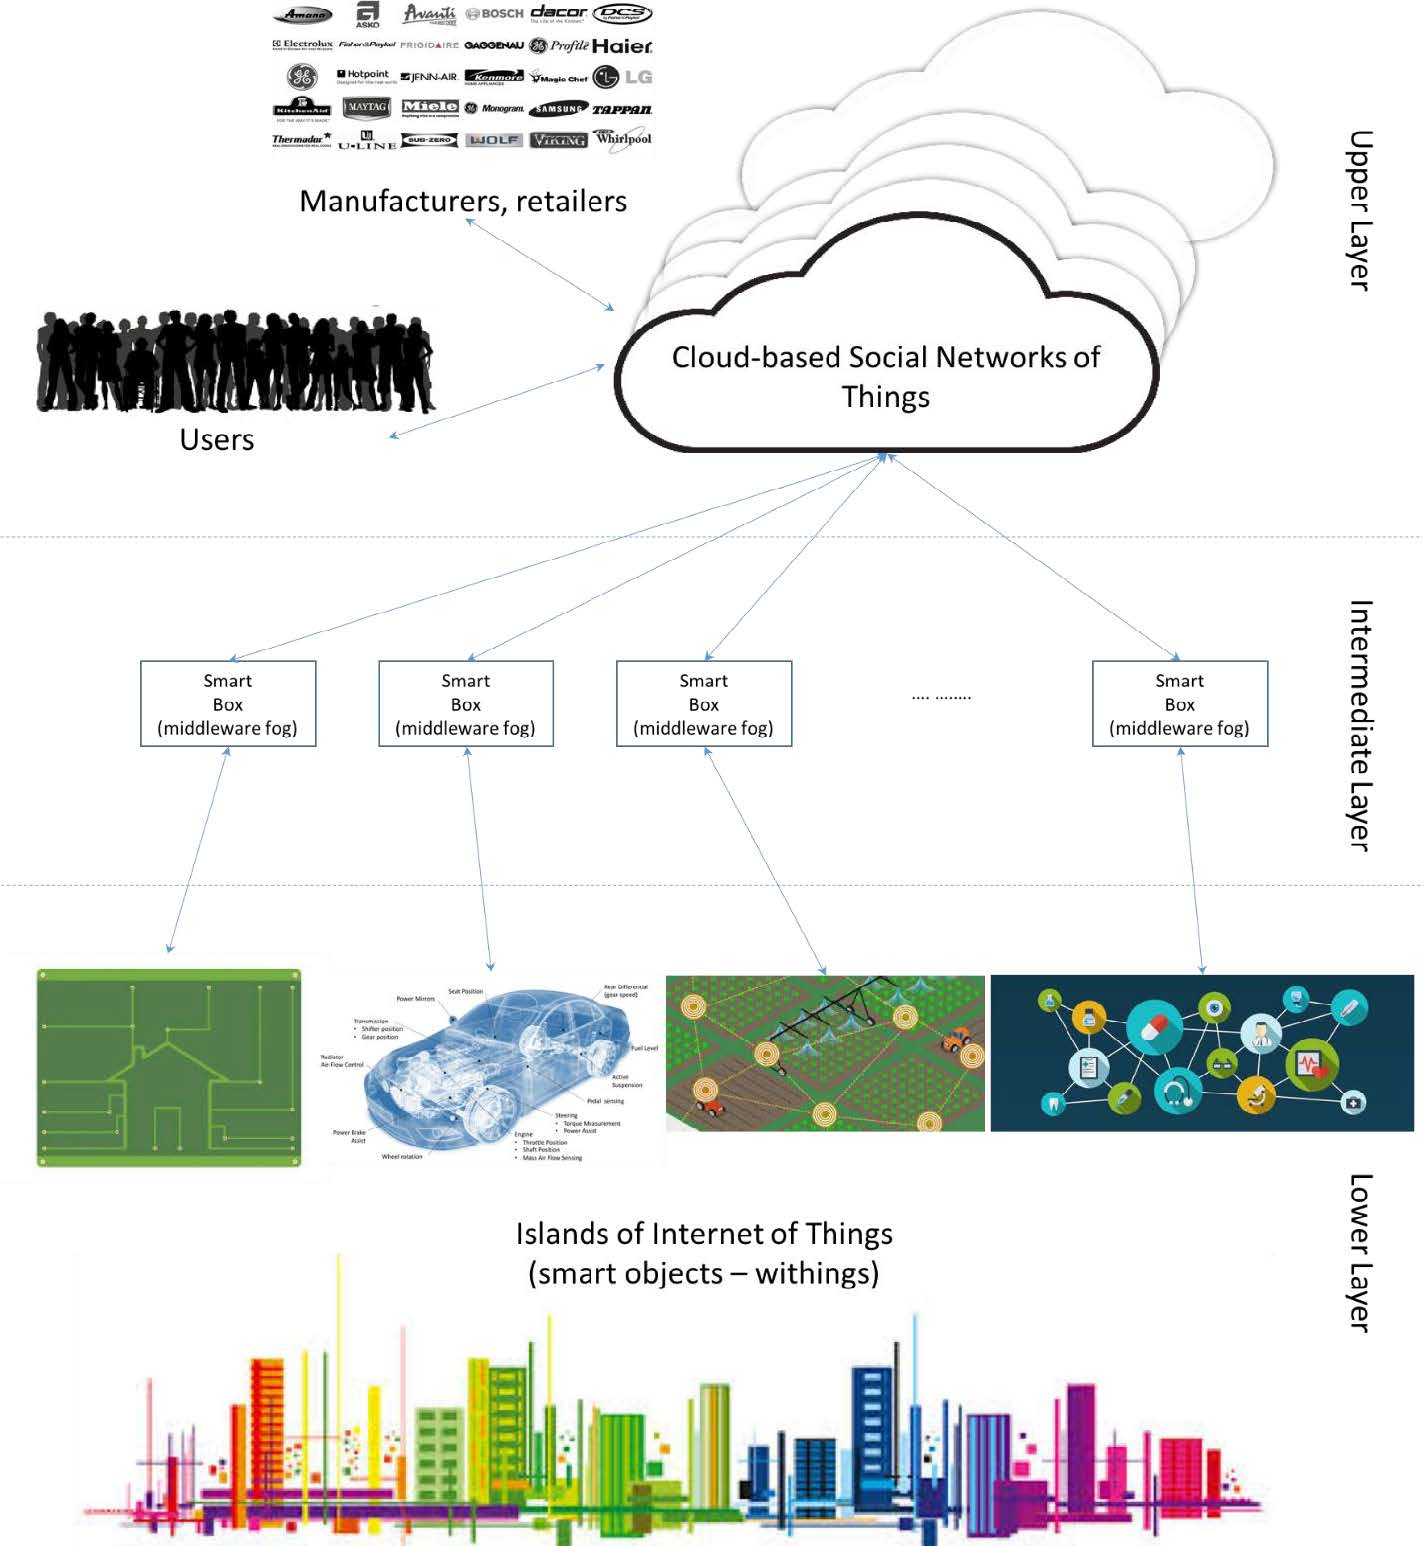
\includegraphics[width=0.48\textwidth]{./fig2-3.jpg}}
	\vspace{-3mm} \caption{\small Contexts (devices, users, location) and instantiations of HACADAs}
	\label{fig2}
\end{wrapfigure}


(I)  The first setup consists of a set of middleware fogs, located in each smart box/gateway of a smart home or public area, grouped together in an evolving (social-like) network along with profiles of manufacturers, retailers and users/owners. The lower layer is formed by all the real devices/objects (things), such as a fridge, a washing machine, a heater, a TV, a Hi-Fi, etc., where each one is abstracted by what we refer to as WiThing (WiT) for Wireless Thing. The WiT is the first level of the device abstraction and its role is to (1) uniquely identify an object/device (2) represent the object in terms of its properties/functionalities through an MIB (Management Information Base), and (3) constitute a bidirectional interface for all communications between the object and the middleware fog located in the smart box/gateway. The intermediate layer contains the smart box/gateway where the middleware fog is implemented. The latter is composed of an ensemble of interconnected modules that will govern all the requests issued by the user through a proper front-end application. To this end, this smart box must interface with any object/device it meets in the surroundings, i.e., any virtual device communicated by the real objects/devices. The upper layer illustrates the complexity of the different couplings to form ensembles of (networks of) manufacturers, retailers and users/owners with the generic representations of their objects/devices.
%%%It consists of a large database with an enquiry system based on sophisticated algorithms.




(II) The second setup complements the previous one in terms of inter-contexts couplings and dynamic formations (and dissolution) of corresponding instances of ensembles with heterogeneous participants. In terms of notation in Figure 1. this can be explained by the following consideration:
(a) If we have an instance of a ``network'' of particular devices (e.g., a washers) from a collection of residential units, depending on the geographical context we may want to compose instances of collections corresponding a group of same devices but operating in a group of buildings in a near-downtown area.
(b) Complementary to this, we may need to couple the ``entity'' corresponding to the ensemble of washers in different units in an apartment complex, with the one of entertainment devices in the same and/or neighboring buildings.


One could readily generalize this in other/multiple contexts -- e.g., the instances representing the traffic-density in different geographical regions may be tied with the crime-rate in those and/or near-by regions and with the ones corresponding to activities of electronic devices in the police cars. %%However, after a certain time of the day/night, such (meta)Avatars may cease to exist.



To enable such situational awareness that is flexible enough to incorporate the dynamic formation of instances that can span not only from networks of users to network of heterogeneous devices, but also through the existence of ensembles comprised of different contextual impacts (space, time, objective to be optimized, etc.) we  propose the concept of Heterogeneity And Context Aware Dynamic Avatars (HACADA) illustrated in Figure~\ref{fig2}. We note that, in addition to the scenario-oriented discussions above, the HACADA's may be created, updated/modified and ceased based on different criteria: (a) particular cyber-properties: e.g., status of network infrastructure, privacy constraints, etc.; (b) Logical or semantical properties which may entail dynamically forming (and dissolving) hierarchies of HACADAs; (c) ``expiration'' of certain criteria (e.g., past 10PM) enabling the leftover descriptors in two different HACADA-instances to be merged into one.


\noindent {\bf Intellectual Merits:}

Throughout this complex environment, and in order to automate the deployment and control, as well as optimize the use of such ensembles of HACADAs comprising multiple instances of operational Internet of Things,
a plethora of issues in data collection and processing (representation, distributed allocation and querying, and information fusion), knowledge discovery, and security and privacy need to be investigated in unified framework. We assert that  such integrated large scale effort, involving researchers from diverse backgrounds, is necessary to  enable exploiting the full potential of the Internet of Things technology  and make it ubiquitous of use. The proposed project has the following list of collaborative research activities as its main Intellectual Merits:

-- {\it Design and development of novel techniques and abstractions for acquisition and representation of data from IoT devices and users}: What separates the HACADAs from both managing and integration of traditional distributed heterogeneous datasets is that, in addition to the set of {\it observed data values}, one needs to seamlessly integrate the notion of {\it dynamic states and transitions}. A peculiarity is that the representation of a state and the rules for valid transitions may differ among HACADA instances -- and yet one may need to use two (or more) such distinct instances for a particular query. Towards that, we will identify a collection of key events spanning multiple contexts (space/location, time, device, network-features) and a collection of basic operands with various overloadings to enable collaborative creation of new HACADAs, merging of existing ones into an instance of a new category, with different consumption modes regarding the ``parents''. We will also investigate the problem of actual placement (and migration) of the representation of HACADAs, to cater to different analytics and privacy/security objectives. 

-- {\it Development of privacy-preserving analytics to discover hidden correlations and usage patterns and behaviors} {\bf NOTE: mention a summary from the section written by Vladimir and Ashfaq}.

-- {\it Design and development of network protocols to mitigate the DoS and greedy behavior in IoT devices} {\bf NOTE: Alek and Farid section-summary}


-- {\it Development of simulation platform as well as real-world testbed of heterogeneous IoTs (devices and users)}. {\bf NOTE: mention a realization of application scencario(s)}.


\noindent {\bf Broader Impacts}: The salient broader impacts of the proposed project are:

{\bf NOTE: need to expand}

This research effort aims to contribute to the rapid development of national and local capacity to respond to critical events and to develop technology to advance the ability and scope of Internet of Things to detect and monitor events in applications of high priority, such as surveillance and habitat monitoring. The proposed research activity is a multidisciplinary effort involving researchers with expertise in distributed databases, security, and data management and analytics. This work will also contribute to, and complement efforts under way for, the design and management of reliable smart facilities. Leveraging on the existing cooperation between Illinois Institute of Technology, Northwestern University and Rutgers University. The PIs have a long record of working on collaborative research projects and have extensively involved undergraduate students, minority students and women in their research.



The proposed collaborative project will be executed by a team of six highly accomplished researchers and their students from three different institutions, who have expertise in all the complimentary areas relevant to the research activities proposed in this project, including: Human Computer Interface, Machine Learning, Information Systems and Data Sciences, Sensor and Sensor Networking, Security, and Privacy. The PI and Co-PIs have a long and well established record of collaborating on different federal government and industry funded  research projects. In the following we provide a brief introduction of the PIs and their relevant expertise.
\begin{itemize}
\vspace{-3mm} \item Ashfaq Khokhar, Illinois Institute of Technology: Wireless Sensor Networks, Data Mining, Cloud Computing
\vspace{-3mm} \item Farid Nait-Abdesselam, Illinois Institute of Technology: Network Security, Wireless Sensor Networks
\vspace{-3mm} \item Mubbasir Kapadia, Rutgers University: Human Computer Interface, Virtual Human Systems
\vspace{-3mm} \item Vladimir Pavlovic, Rutgers University: Machine Learning, Dynamic System Modeling, Computer Vision
\vspace{-3mm} \item Aleksander Kuzmanovic, Northwestern University: Networks Security, Denial-of-service Resiliency, Content Distribution
\vspace{-3mm} \item Goce Trajcevski, Northwestern University: Moving Objects Databases,Data Management in Sensor Networks
\end{itemize}


